\section{Ejercicios sobre Gramáticas de Atributos}
La gramática:
\begin{verbatim}
axioma         ::= USUARIO peliculas
peliculas      ::= peliculas peliculas | pelicula
pelicula       ::= TITULO valoraciones
valoraciones   ::= valoraciones valoracion valoracion
valoracion     ::= (USUARIO:NUMERO)
\end{verbatim}
genera frases que consisten en una secuencia de películas con sus respectivas valoraciones realizadas por los usuarios.Al principio de las frases generadas por la
gramática siempre aparece el nombre de un usuario. A continuación se muestran tres ejemplos:

jaime Star\_Wars(jaime:10)(ana:10) Spiderman(ana:10)(pepe:1)

ana Kapax(pepe:100)(jaime:1) Avatar(ana:40) Pi(pepe:100)(ana:1)

mike Kapax(pepe:100)(jaime:1) Avatar(ana:40) Pi(pepe:100)(ana:1)


Se desa añadir a esta gramática un sistema de atributos que haga lo siguiente:
\begin{enumerate}
\item Calcular el número total de películas valoradas
\item Indicar el título y la valoración de la película mejor valoradas por el usuario indicado al principio de la cadena. Si no hay ninguna películas valorada por dicho usuario debe indicarse tal circunstancia.
\end{enumerate}

Por ejemplo, para las tres cadenas anteriores se mostrarían respectivamente los mensajes siguientes:

Se han valorado 2 películas.
La mejor valorada por jaime es Star\_Wars, con una valoración de 10.

Se han valorado 3 películas.
La mejor valorada por ana es Avatar, con una valoración de 40.

Se han valorado 3 películas.
Ninguna película ha sido valorada por mike.


\textbf{Notas:}
\begin{itemize}
\item Puede considerarse que existe un proceso de análisis morfológio que asigna a los símbolos terminales los siguientes atributos semánticos: USUARIO.nombre (nombre de usuario), TITULO.titulo (título de la película), NUMERO.valor (valor numérico del número)
\item Debe comprobarse que el usuario que aparece al principio de la cadena no valora más de una vez la misma película. No es necesario realizar esta comprobación para el resto de usuarios.
\item No está permitido el uso de información global
\item Debe responderse a cada una de las cuestiones usando las plantillas correspondientes
\end{itemize}
\newpage

\begin{problem}[1]
Describa explícita y brevemente el significado de cada atributo que utilice, así como el proceso de actualización de cada uno de ellos mencionando si se realiza herencia o síntesis en su propagación. Responde rellenando la tabla:
\solution
\begin{tabular}{|c|c|l|}
\hline
SÍMBOLO & ATRIBUTOS & DESCRIPCIÓN \\
\hline
\hline
USUARIO & nombre & Nombre del usuario.\\
\hline
TITULO & titulo & Título de la película.\\
\hline
NÚMERO & valor & Valor numérico del número.\\
\hline
valoración & nota & nota de la valoración (por síntesis) \\
\cline{2-3}
& usuario & usuario que da la valoración (por síntesis)\\
\hline
valoraciones & usuario\_actual & Usuario inicial (por herencia)\\
\cline{2-3}
& notaMax & nota máxima (por síntesis) \\
\hline
& nota & Nota máxima de la película (por síntesis)\\
\cline{2-3}
película & titulo & titulo de la película (por síntesis) \\
\cline{2-3}
& usuario\_actual & Usuario inicial (por herencia) \\
\hline
& num & Número de películas valoradas (por síntesis)\\
\cline{2-3}
películas & usuario\_actual & Usuario inicial (por herencia) \\
\cline{2-3}
& titulo & titulo de la película mejor valorada (por síntesis) \\
\cline{2-3}
& nota & nota de la película mejor valorada (por síntesis)\\
\hline
\end{tabular}
\end{problem}

\begin{problem}[2]
Define formalmente la gramática utilizando la notación explicada en el temario de esta asignatura. Utiliza la siguiente tabla, en la que debes indicar, para cada regla de la gramática, las acciones semánticas asociadas junto con el instante en que se deben ejecutar.
\solution
\begin{tabular}{|c|l|}
\hline
INSTATE & ACCIÓN \\
\hline
\multicolumn{2}{|l|}{axioma ::= USUARIO peliculas} \\
\hline
 1 & peliculas.usuario\_actual = USUARIO.nombre \\
\hline
 2 & print("Se han valorado " + peliculas.num + " películas") \\
 & print("la mejor valorada por " + USUARIO.nombre + " es " + peliculas.titulo \\ & + " con una valoración de " + peliculas.nota + ".")\\
 \hline
\multicolumn{2}{|l|}{peliculas\_1 ::= peliculas\_2 pelicula} \\
\hline
 0 & peliculas\_2.usuario\_actual = peliculas\_1.usuario\_actual \\ & pelicula.usuario\_actual = peliculas\_1.usuario\_actual\\
 \hline
 2 & if(peliculas\_2.nota>pelicula.nota)\{\\ &
 peliculas\_1.nota=peliculas\_2.nota\\ &
 peliculas\_1.titulo=peliculas\_2.titulo\}\\ &
 else\{peliculas\_1.nota=pelicula\_1.nota\\ &
 peliculas\_1.titulo=pelicula\_1.titulo\}\\ &
 peliculas\_1.num = peliculas\_2.num+1\\
\hline
\multicolumn{2}{|l|}{peliculas ::= pelicula} \\
\hline
 0 & pelicula.usuario\_actual = peliculas.usuario\_actual \\
 \hline
 1 & peliculas.titulo = pelicula.titulo \\ & peliculas.nota = pelicula.nota \\ &
 peliculas.num=1\\
\hline
\multicolumn{2}{|l|}{pelicula ::= TITULO valoraciones} \\
\hline
0 & valoraciones.usuario\_actual = pelicula.usuario\_actual \\
 \hline
 1 & pelicula.titulo = TITULO.titulo \\
 \hline
 2 & pelicula.nota=valoraciones.notamax\\
\hline
\multicolumn{2}{|l|}{valoraciones\_1 ::= valoraciones\_2 valoracion} \\
\hline
0 & valoraciones\_2.usuario\_actual = valoraciones\_1.usuario\_actual\\
\hline
2 & if(valoraciones\_1.usuario\_actual==valoracion.usuario AND valoraciones\_2.notamax\\& $\neq$ 0)\{\\ &
print("ERROR")\\&
\}else if(valoraciones\_1.usuario\_actual==valoracion.usuario)\}\\&
valoraciones\_1.notamax=valoracion.nota\\&
\}else if(valoraciones\_2.notamax $\neq$0)\{\\&
valoracion\_1.notamax=valoraciones\_2.notamax\\&
\}else\{valoraciones\_1.notamax=0\}\\
\hline
\multicolumn{2}{|l|}{valoraciones ::= valoracion} \\
\hline
 0 & valoraciones.notamax=0 \\
 \hline
 1 & if(valoraciones.usuario\_actual==valoracion.usuario)\{\\ &
 valoraciones.notamax=valoracion.nota\}\\
\hline
\multicolumn{2}{|l|}{valoracion ::= (USUARIO:NUMERO)} \\
\hline
 2 & valoracion.nota = NUMERO.valor\\ & valoracion.usuario=USUARIO.nombre\\
 \hline

\end{tabular}


Lo de votosUs se podría hacer declarando otro atributo de error a peliculas en caso de que se superen esos votos
\end{problem}

\begin{problem}[3]
La tabla que aparece a continuación representa el árbol de derivación para la siguiente sentencia:
\begin{verbatim}
jaime Star_Wars(jaime:10)(ana:30) Spiderman(ana:10)(jaime:20)
\end{verbatim}
Nótese que, para simplificar, se están ignorando los terminales (, : y ) en la regla para el no terminal valoracion. Muestra, sobre la tabla, los valores de los atributos semánticos y alguna indicación gráfica que indique cómo se realiza la propagación.
\solution
\newpage

\includepdf[pages={5}, angle=90]{tex/ejerciciosHoja2/Hoja2_2014_10_08.pdf}
\newpage

\end{problem}

\begin{problem}[4]
Considérese la siguiente gramática independiente del contexto:
\begin{verbatim}
axioma        ::= DINERO lista_compra
lista_compra  ::= compra lista_compra | compra
compra        ::= [PRODUCTO, PRECIO]
\end{verbatim}
Esta gramática genera sentencias que consisten en una cantidad de DINERO seguida de una lsita de compras, cada una con un PRODUCTO y el PRECIO del mismo. Tanto el DINERO como el PRECIO son números reales.

Se desa añadir a esta gramática un sistema de atributos que compruebe si se puede hacer la compra con el dinero disponible. Se indicarán los productos de la lista que se pueden comprar y el saldo disponible al final. Se supone que los productos se adquieren en el mismo orden en el que aparecen en la lista.

\textbf{Notas:}
\begin{itemize}
\item Puede considerarse que existe un proceso de análisis morfológico que asigna a los símbolos terminales los siguientes aributos semánticos: PRODUCTO.nombre (nombre del producto), PRECIO.valor (valor numérico del precio) y DINERO.valor (valor numérico del dinero).
\item No está permitido el uso de información global
\end{itemize}
\solution

\begin{tabular}{|c|c|l|}
\hline
SÍMBOLO & ATRIBUTOS & DESCRIPCIÓN \\
\hline
\hline
DINERO & valor & Valor numérico del dinero. \\
\hline
PRECIO & valor & Valor numérico del precio. \\
\hline
PRODUCTO & nombre & Nombre del producto. \\
\hline
 lista\_compra & valorTotal & valor numérico de toda la compra. \\
 \cline{2-3}
  & dinero & dato de dinero con diferentes utilidades  \\
\hline
compra & valor & valor de la compra \\

\hline
\end{tabular}

\begin{tabular}{|c|l|}
\hline
INSTATE & ACCIÓN \\
\hline
\multicolumn{2}{|l|}{axioma ::= DINERO lista\_compra} \\
\hline
 0 & print("Disponible: " + DINERO.valor) \\ & lista\_compra.valorTotal = 0\\
 \hline
 2 &
  print("Total: " + lista\_compra.valorTotal) \\ &
  print("Saldo: " + lista\_compra.dinero)\\
 \hline
\multicolumn{2}{|l|}{lista\_compra\_1 ::= compra lista\_compra\_2} \\
\hline
 1 & lista\_compra\_1.valorTotal = lista\_compra\_2.valorTotal + compra.valor \\
\hline
\multicolumn{2}{|l|}{lista\_compra ::= compra} \\
\hline
 1 & lista\_compra.valorTotal = lista\_compra.valorTotal + compra.valor. \\
\hline
\multicolumn{2}{|l|}{compra ::= [PRODUCTO,PRECIO](NOTA:omitimos corchetes y coma en los instantes)}\\
\hline
2 & compra.valor=PRECIO.valor \\ & print(PRODUCTO.nombre + " : " + PRECIO.valor)\\
\hline

\end{tabular}


\end{problem}

\begin{problem}[5]
Considérese la siguiente gramática independiente del contexto:2
\begin{verbatim}
romano ::= IList | I V | V IList
IList  ::= IList I | λ
\end{verbatim}
Esta gramática genera sentencias entre las que se encuentran los números romanos hasta el 8.

Se pide añadir a la gramática un sistema de atributos que compruebe si la sentencia corresponde a un número romano correcto y, en caso afirmativo, imprima su valor numérico.

\textbf{No está permitido el uso de información global}
\solution

\begin{tabular}{|c|c|l|}
\hline
SÍMBOLO & ATRIBUTOS & DESCRIPCIÓN \\
\hline
 & valor & Valor numérico del número. \\
\cline{2-3}
IList & ies & Número de ies que tiene \\
\cline{2-3}
 & cadena & String con el número romano \\
\hline
 
\end{tabular}

\begin{tabular}{|c|l|}
\hline
INSTATE & ACCIÓN \\
\hline
\multicolumn{2}{|l|}{romano ::= IList} \\
\hline
 0 & IList.valor=0\\ & IList.ies=0 \\ & IList.cadena=""\\
 \hline
\multicolumn{2}{|l|}{romano ::= I V} \\
\hline
 0 & print("IV, número romano correcto, su valor es 4")\\
\hline
\multicolumn{2}{|l|}{romano ::= V IList} \\
\hline
 0 & IList.valor=5\\ &  IList.ies = 0\\ & IList.cadena="V"\\
\hline
\multicolumn{2}{|l|}{Ilist\_1 ::= Ilist\_2 I}\\
\hline
 0 & IList\_2.valor = IList\_1.valor + 1\\ & IList\_2.ies= IList\_1.ies+1\\ & IList\_2.cadena = IList\_1.cadena + "I"\\
\hline
\multicolumn{2}{|l|}{Ilist ::= $\lambda$}\\
\hline
0 & if(IList.ies<4) \\& print(IList.cadena + ", número romano correcto, su valor es " + IList.valor) \\ & else print(IList.cadena + ", no es un número romano correcto)\\
\hline


\end{tabular}

\end{problem}

\begin{problem}[6]
Considérese la gramática independiente del contexto resultante de añadir a la del ejercicio 5 el siguiente axioma:
\begin{verbatim}
S ::= romanod = IList
\end{verbatim}
Esta gramática genera sentencias formadas por dos cadenas separadas por el signo '='. La primera cadena es igual que las generadas por la gramática del ejercicio 5. La segunda cadena es una lista de símbolos I.

Se pide añadir a la gramática un sistema de atributos que compruebe si, en el caso de que la primera cadena sea un número romano correcto, el valor del mismo coincide con el número de símbolos I en la segunda cadena.

\textbf{No está permitido el uso de información global}
\solution
\begin{tabular}{|c|c|l|}
\hline
SÍMBOLO & ATRIBUTOS & DESCRIPCIÓN \\
\hline
romano & valor & valor numérico del numero romano\\
\hline
 & valor & Valor numérico del número. \\
\cline{2-3}
IList & ies & Número de ies que tiene \\
\cline{2-3}
 & cadena & String con el número romano \\
\hline
 
\end{tabular}

\begin{tabular}{|c|l|}
\hline
INSTATE & ACCIÓN \\
\hline
\multicolumn{2}{|l|}{S ::= romano = IList} (NOTA: ignoramos el signo igual al contar instantes) \\
\hline
 2 & if(romano.ies<4)\{\\ & 		if(IList.valor = romano.valor) print("coincide con segunda cadena")\\ & else print("no coincide con segunda cadena") \}\\
 \hline
\multicolumn{2}{|l|}{romano ::= IList} \\
\hline
0 & IList.cadena="" \\
\hline
 1 & romano.ies = IList.ies \\ & romano.valor=IList.valor\\ & if(romano.ies<4) print(", número romano correcto, su valor es" +romano.valor)\\ & else print(", no es un número romano correcto")\\
 \hline
\multicolumn{2}{|l|}{romano ::= I V} \\
\hline
 0 & romano.valor=4 \\ & romano.ies = 1 \\ & print("IV")\\
 \hline
\hline
\multicolumn{2}{|l|}{romano ::= V IList} \\
\hline
 0  & IList.cadena="V"\\
 \hline
 2 & romano.ies = IList.ies\\
 & romano.valor= IList.valor + 5\\
\hline
\multicolumn{2}{|l|}{Ilist\_1 ::= Ilist\_2 I}\\
\hline
 0 & IList\_2.cadena = IList\_1.cadena + "I"\\
 \hline
 2 & IList\_1.valor = IList\_2.valor + 1\\ & IList\_1.ies= IList\_2.ies+1\\
\hline
\multicolumn{2}{|l|}{Ilist ::= $\lambda$}\\
\hline
0 & print(IList.cadena)\\
\hline


\end{tabular}

\end{problem}
\end{document}
